\graphicspath{{../05QuantumPhysics/pics/}}

\chapter{Quantum Physics}\label{ch:QuantumPhysics}
\lettrine[lines=2]{\color{darkocre}T}{he} first type of operators -- and
corresponding tensors -- that we encountered has a simple type:
\[
\op{L}\,\vec{a} = \vec{b}\,.
\]
It is a linear unary function mapping vectors into vectors.


\begin{myprereq}{Prerequisite Knowledge}
To fully understand the material of this chapter, readers should be comfortable with the following concepts:

\begin{itemize}
	\item \phantom{phantom}
	\vspace{-0.5cm}
	\item State
	\item Dynamical equations
\end{itemize}	
\end{myprereq}

\section{Quantum System}\label{sec:QuantumSystem}
We are looking for a binary operator $\op{\sigma}$ that yields a number
based on two vectors:
\[
\ketbra{\sigma}{\sigma}\,\vec{a}\,\vec{b}=x\,.
\]

\section{Quantum State}\label{sec:QuantumState}
We are looking for a binary operator $\op{\sigma}$ that yields a number
based on two vectors:
\[
\ketbra{\sigma}{\sigma}\,\vec{a}\,\vec{b}=x\,.
\]
\subsection{States Overlap}
\[
\braket{\psi}{\phi}.
\]

\section{Quantum Dynamics}\label{sec:QuantumDynamics}
We are looking for a binary operator $\op{\sigma}$ that yields a number
based on two vectors:
\[
\ketbra{\sigma}{\sigma}\,\vec{a}\,\vec{b}=x\,.
\]

\section{Quantum Hamiltonian}\label{sec:QuantumHamiltonian}
We are looking for a binary operator $\op{\sigma}$ that yields a number
based on two vectors:
\[
\ketbra{\sigma}{\sigma}\,\vec{a}\,\vec{b}=x\,.
\]


\section{Quantum Bit}\label{sec:Qubit}
Any quantum system with two active states is called a \emph{qubit}. The state with lower energy is usually called \emph{ground state} and denoted as $\ket{g}$ or $\ket{0}$ (zero). The state with higher energy is usually called \emph{excited state} and denoted as $\ket{e}$ or $\ket{1}$ (one). The notation $\ket{0}\,,\ket{1}$ is used in the field of quantum information and computation.

If the energy of the ground and excited states are $E_g$ and $E_e$, respectively, then the Hamiltonian of a qubit can be written using projectors
\[
\op{H} = E_g\ketbra{g}{g}+E_e\ketbra{e}{e}\,.
\]
It requires an energy $\Delta E=E_e-E_g$ to excite the qubit from the lower energy state to the higher energy state. This energy may come from a quantum of electromagnetic field oscillating with frequency $\omega=\Delta E/\hbar$.

\subsection{Flipping Operator}
Transition between the states of a qubit can be described mathematically using operators that map one state into another. For example, an operator $\op{F}$ that \emph{flips} states must do the following:
\[
\op{F}\,\ket{0}=\ket{1}\,,\quad \op{F}\,\ket{1}=\ket{0}\,.
\]
Such operator can be easily built from the tensor products:
\[
\op{F} = \ketbra{1}{0}+\ketbra{0}{1}\,.
\]
Each term in this sum is useful in quantum theory. The first term is called \emph{raising operator} and is denoted as 
$ \op{\sigma}_\plus=\ketbra{1}{0}$. The second term is called \emph{lowering operator} and is denoted as $ \op{\sigma}_\minus=\ketbra{0}{1}$. Apparently, the raising operator excites the qubit from the ground state, while the lowering operator brings the qubit down from the excited state.
\begin{exercise}
	Calculate $\op{F}^2$.
\end{exercise}
\begin{exercise}
	Calculate (a) $\op{\sigma}_\plus \op{\sigma}_\plus$; (b) $\op{\sigma}_\minus \op{\sigma}_\minus$; (c) $\op{\sigma}_\plus \op{\sigma}_\minus$; (d) $\op{\sigma}_\minus \op{\sigma}_\plus$.
\end{exercise}

\begin{exercise}
	Show that  $\op{\sigma}_\plus \op{\sigma}_\minus+\op{\sigma}_\minus \op{\sigma}_\plus=\op{I}$, where $\op{I}$ is the identity operator.
\end{exercise}

\begin{exercise}
	Show that the qubit Hamiltonian can be written in terms of the raising and lowering operators as follows:
	
	\[
	\op{H} = \hbar\omega\left(\op{\sigma}_\plus \op{\sigma}_\minus+\epsilon\op{I} \right)\,,
	\]
	where $\epsilon=E_g/\Delta E$.
\end{exercise}

\subsection{Number Operator}
The operator $\op{n}=\op{\sigma}_\plus \op{\sigma}_\minus$ is called \emph{number operator} for the following reason. First, note that $\op{\sigma}_\plus \op{\sigma}_\minus=\ketbra{1}{1}$ is the projector on the excited state of qubit.
\begin{figure}[htbp]
	\centering
	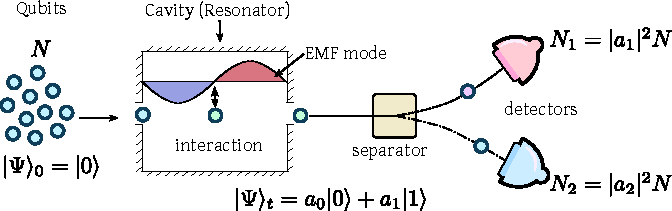
\includegraphics[scale=1.0]{qubitNumberOperatorMeaning}
	\caption{Qubits initially in the ground state $\ket{0}$ travel through a cavity resonator with an electromagnetic field mode attuned to the qubits transition energy $\Delta E=\hbar\omega$. After interaction, the state of each qubit changes to $\ket{\Psi_t}$. Then the qubits are "measured"/separated into two groups, based on their final state.}
	\label{fig:qubitNumberOperatorMeaning}
\end{figure}

Next, consider an experiment schematically shown in Figure \ref{fig:qubitNumberOperatorMeaning}. In this experiment a large number $N$ of qubits start in the ground state $\ket{0}$ and go through a region (cavity) where they can interact with an oscillating electromagnetic field (mode). After leaving the cavity, each qubit goes through a special device which splits the beam into two parts, depending on the measured state of a qubit. The top detector detects $N_1$ qubits in state $\ket{1}$, the bottom detector detects $N_2$ qubits in ground state. The $N_1$  qubits correspond to the number of energy quanta absorbed from cavity. This number can be expressed as
\[
N_1=N |a_1|^2=N\bra{\Psi_t}\op{n}\ket{\Psi_t}\,.
\]  
In other words, the expectation value of the operator $\op{n}$ determines the number of energy quanta absorbed from the mode of electromagnetic field inside the cavity.
 

\section{Quantum Oscillator}\label{sec:QuantumOscillator}
The \emph{principle of the quantization of action} can be applied to harmonic oscillator. The result is the quantization of energy levels. 

The energy of a harmonic oscillator can be expressed in terms of the maximum momentum $p_m$ or in terms of the maximum displacement $x_m$:
\[
H = \frac{p_m^2}{2m}\quad\textrm{ or }\quad H=\frac{kx_m^2}{2}\,.
\]
Multiplying these two equalities and recalling that $\omega^2=k/m$, we obtain
\[
H = \frac{\omega x_m p_m}{2}\,.
\]
The path which the state vector $\ket{\xi}=(x,p)$ follows in phase space is an ellipsis with the major semi-axes $x_m$ and $p_m$. The area of this ellipsis is $A=\pi x_m p_m$. Therefore, the connection between the energy of harmonic oscillator and the area is given by
\[
H=\frac{\omega}{2\pi}A\,.
\]
The area $A$ is a physical quantity with the units of action.

As shown in Figure \ref{fig:phaseSpaceQuantum}(a), areas in phase space have the smallest size limited by the elementary quantum of action $h$ -- known as Planck constant. The quantization of action and, consequently, the quantization of phase-space area, has two important implications for harmic oscillator.
\begin{figure}[htbp]
	\centering
	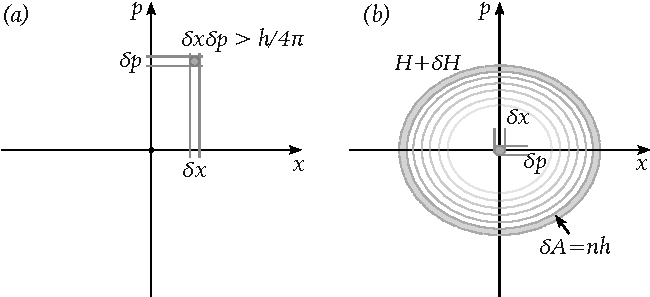
\includegraphics[scale=1.0]{phaseSpaceQuantum}
	\caption{Areas of phase-space regions have the units of action. Quantization of action implies quantization of phase-space area. (a) The smallest area in phase space is limited by the fundamental quantum of action $h$ -- Planck's constant. (b) Area of the ellipsis inside the path of harmonic oscillator is proportional to its energy. Quantization of area leads to the quantization of energy of harmonic oscillator.}
	\label{fig:phaseSpaceQuantum}
\end{figure}

First, every time an oscillator absorbs some energy $\Delta E$, the maximum deviation and the maximum momentum increase. The ellipsis in phase space increases its area. But since the area in phase space can't grow continiously--changes in discrete quanta $\delta A=h$--we must have discreete changes in energy. Second, the existence of the elementary quantum of action and the smallest are in phase space, require that the lowest energy state of harmonic oscillator is described not by a point in phase space, but by an elementary ellipsis such that $A_0=\delta x\delta p\propto h$. Putting these two ideas together, we conclude that the area of the ellipsis can be written as
\[
A_n = A_0 + nh\,.
\]
The energy of the oscillator then takes the form
\[
H=n\hbar\omega + E_0\,,
\]
where $\hbar=h/2\pi$ is called \emph{reduced Planck's constant}, and $E_0$ is the lowest energy of the harmonic oscillator. From the expression for $H$ follows that harmonic oscillator can be in a countable set of states, growing in energy from $E_0$ by a fixed step $\hbar\omega$. 

The energy of the lowest state can be written in terms of the step size $\hbar\omega$: $E_0=e_0\hbar\omega$, where $e_0$ is some number (it will be found later). Finally, we can write the energy of harmonic oscillator as follows:
\[
H=\hbar\omega(n + e_0)\,.
\]

\subsection{Hamiltonian Operator}
For any quantum system with descrete energy states $E_0, E_1, E_2,\ldots, E_n\ldots$ the Hamiltonian operator can be written in terms of projectors:
\[
\op{H}=\int E_k\ketbra{k}{k}\,,\quad k=0,1,2,\ldots,n\ldots 
\]
For harmonic oscillator $E_k=E_0+k\hbar\omega$ for $n>1$ and the Hamiltonian operator can be written as follows
\[
\op{H} = \int (E_0+k\hbar\omega)\ketbra{k}{k}\,.
\]
The number $k$ tells how many excitations quantum oscillator absorbed to reach the energy state $\ket{k}$.
Opening the parentheses and recalling that
\[
\int\ketbra{k}{k}=\op{I}\,,
\] 
we obtain 
\[
\op{H} = E_0\op{I}+\hbar\omega \int k\ketbra{k}{k}\,.
\]
This expression is very similar to the Hamiltonian of a qubit 
\[
\op{H}_{qb}=E_g\op{I}+\hbar\omega\op{n}
\]
where $\op{n}=\op{\sigma_\plus}\op{\sigma_\minus}$ is a number operator. The similarity is not accidental, as the operator $\op{n}=\int k\ketbra{k}{k}$ plays the role of the number operator. Indeed, it is easy to check by direction application that:
\[
\op{n}\,\ket{n}=n\ket{n}\,.
\]
In other words, the energy states $\ket{n}$ of harmonic oscillator, are the eigen-states of the number operator $\op{n}$ with the eigen-value $n$ corresponding to the number of excitation level.
\begin{exercise}
	Prove that $\op{n}\,\ket{n}=n\ket{n}$ by direction application of the operator $\op{n}=\int k\ketbra{k}{k}$.
\end{exercise}

The expression for the number operator $\op{n}$ can be obtained in a different way. First note that
\[
\op{H}\,\ket{n}=E_n\ket{n}\,,\quad\textrm{ where } E_n = E_0 + n\hbar\omega\,.
\]
From this follows
\[
(\op{H}-E_0\op{I})\,\ket{n}=n\hbar\omega\,\ket{n}\,,
\]
and, consequently, 
\[
\frac{(\op{H}-E_0\op{I})}{\hbar\omega}\,\ket{n}=n\,\ket{n}\,.
\]
The operator on the left hand side of this equation is the number operator $\op{n}$. It can be simplified once we recall that
\[
\op{H}=\int E_k\ketbra{k}{k}\quad\textrm{ and }\quad \op{I}=\int\ketbra{k}{k}\,.
\]
Using these relations, we first write
\[
\op{H}-E_0\op{I}=\int (E_k-E_0)\ketbra{k}{k}\,.
\]
Then, remembering that $E_k=E_0+k\hbar\omega$, we immediately arrive at
\[
\op{n}=\frac{(\op{H}-E_0\op{I})}{\hbar\omega}=\int k\ketbra{k}{k}\,.
\]
Thus, the operator of quantum harmonic oscillator can be written in the following form:
\[
\op{H}_{osc}=E_0\op{I}+\hbar\omega\op{n}\,.
\]
\subsection{Ladder Operators}
The number operator for qubit could be expressed as the product of two simple operators that raised or lowered qubit states:
\[
\op{n} = \op{\sigma}_\plus\op{\sigma}_\minus\,.
\]
The idea of raising and lowering states is also applicable to harmonic oscillator. Similar to qubit, we can write such operators as tensor products:
\[
\op{a}_\plus = \ketbra{n+1}{n}\textrm{ and }\quad\op{a}_\minus=\ketbra{n-1}{n}\,.
\]
Unfortunately, these operators will act properly only on the state $\ket{n}$.
\begin{exercise}
	Evaluate (a) $\op{a}_\plus \,\ket{n}$; (b) $\op{a}_\minus \,\ket{n}$; (c) $\op{a}_\plus \,\ket{n+m}$; (d) $\op{a}_\plus \,\ket{n+m}$.
\end{exercise}
It is easy to fix this problem by summing over all states:
\[
\op{a}_\plus=\int \ketbra{k+1}{k}\quad\textrm{ and }\quad \op{a}_\minus=\ketbra{0}{0}+\int \ketbra{m-1}{m}\,,\quad m > 0\,.
\]
The first term in the expression for $\op{a}_\minus$ ensures that the vacuum state remains unchanged: $\op{a}_\minus\,\ket{0}=\ket{0}$.
\begin{exercise}
	Evaluate (a) $\op{a}_\plus \,\ket{n}$; (b) $\op{a}_\minus \,\ket{n}$.
\end{exercise}
Let's check whether $\op{a}_\plus\op{a}_\minus$ yields the number operator $\op{n}=\int k\ketbra{k}{k}$. Even without explicitely evaluating the composition $\op{a}_\plus\op{a}_\minus$ we can see that it is unlikely to contain the required factor $k$.
\begin{exercise}
	Show that $\op{a}_\plus\op{a}_\minus=\ketbra{1}{0}-\ketbra{0}{0}+\op{I}$.
\end{exercise}

To find better operators for raising and lowering states of harmonic oscillator, we can taken a closer look at the qubit case. There we had $\op{\sigma}_\plus\,\ket{0}=1\ket{1}$ and $\op{\sigma}_\minus\,\ket{1}=1\ket{0}$\,. We explicitely added "1" in front of the final states, to highlight the following property of the $\op{\sigma}$-operators:
\[
\op{\sigma}_\plus\,\ket{k}=\sqrt{k+1}\ket{k+1}\quad\textrm{ and } \op{\sigma}_\minus\,\ket{k}=\sqrt{k}\ket{k-1}\,.
\]
Thus, we can "upgrade" the raising and lowering operators $\op{a}_\plus$ and $\op{a}_\minus$ to include the information about the state they act on. We want them to behave as follows:
\[
\op{a}_\plus\,\ket{k}=\sqrt{k+1}\ket{k}\quad\textrm{ and }\quad \op{a}_\minus\,\ket{m}=\sqrt{m}\ket{m-1}\,.
\]
\begin{exercise}
	Evaluate $\left(\op{a}_\plus\right)^p\,\ket{0}$.
\end{exercise}
\begin{exercise}
	(a) Show that the upgraded operators have the property 
	\[
	\op{a}_\plus\op{a}_\minus\,\ket{m}=m\ket{m}\quad m>0\,.
	\]	
	(b) Evalulate $\op{a}_\minus\op{a}_\plus\,\ket{m}$.
\end{exercise}
\begin{exercise}
	(a) Show that 
	\[
	\op{a}_\minus\op{a}_\plus-\op{a}_\plus\op{a}_\minus=\op{I}\,.
	\]	
\end{exercise}

Such raising and lowering operators (also called \emph{ladder operators}) are very useful when working with quantum harmonic oscillators. In terms of the ladder operators, the Hamiltonian of quantum oscillator is written as
\[
\op{H}_{osc} = \hbar\omega\op{n}+E_0\op{I}\,,
\]
where the number operator $\op{n}=\op{a}_\plus\op{a}_\minus$. 


\subsection{Conjugation}
The raising operator $\op{a}_\plus$ can be written in terms of the tensor products:
\[
\op{a}_\plus=\int_0 \sqrt{k+1}\ketbra{k+1}{k}\,.
\]
If we limit the lowering operator to states $\ket{m}$ with $m>0$, then it also allows a simple representation
\[
\op{a}_\minus=\int_1 \sqrt{m}\ketbra{m-1}{m}\,.
\]
By changing the summation variable $m-1=k$ (and, therefore, $m=k+1$), we can re-write the summation over $k=0,1,2\ldots$:
\[
\op{a}_\minus=\int_0 \sqrt{k+1}\ketbra{k}{k+1}\,.
\]
Now the expression for $\op{a}_\minus$ became similar to the expression for $\op{a}_\plus$, with the exception that the order of states in the tensor product is flipped:
\[
\ketbra{k+1}{k}\leftrightarrow \ketbra{k}{k+1}\,.
\]
This change of order of factors in a tensor product is called \emph{conjugation}. The operators $\op{a}_\minus$ and $\op{a}_\plus$ are therefore related to each other via the \emph{conjugation operation}. These operators are said to be \emph{conjugates} of each other. 

The relation of conjugation gives some insight into what the lowering operator $\op{a}_\minus$ does to the vacuum state:
\[
\op{a}_\minus\,\ket{0}=\int_0  \sqrt{k+1}\ket{k}\braket{k+1}{0}=0\int_0\sqrt{k+1}\ket{k}=0\ket{\infty}\,,
\]
where we introduced a vector 
\[
\ket{\infty}=\ket{0}+\sqrt{2}\ket{1}+\sqrt{3}\ket{2}+\ldots+\sqrt{n+1}\ket{n}+\ldots
\]
Obviously, $\ket{\infty}\ne\ket{0}$. The overall factor of zero negates any possible contributions of $\ket{\infty}$, making the product $0\ket{\infty}$ a special "zero vector" $\ket{z_0}$, with the natural property
\[
\ket{k}+\ket{z_0}=\ket{k}\,.
\]
The vector $\ket{z_0}$ does not correspond to any physical state, but represents a mathematical "zero vector". Since for all mathematical manipulations the vectors $0\ket{\infty}$ and $0\ket{0}$ are equivalent,
we can express the action of the lowering operator $\op{a}_\minus$ on the vacuum state as follows:
\[
\op{a}_\minus\,\ket{0}=0\ket{0}\,.
\]
Finally, the action of the number operator $\op{n}=\op{a}_\plus\op{a}_\minus$ on the vacuum state can be evaluated:
\[
\op{a}_\plus\op{a}_\minus\,\ket{0}=\op{a}_\plus(\op{a}_\minus\,\ket{0})=0(\op{a}_\plus\,\ket{0})=0\ket{1}=0\ket{0}\,,
\]
here we used the mathematical equivalence of states $0\ket{1}$ and $0\ket{0}$.

\begin{mybio}{Dagger Notation}
	The relation of conjugation between operators is denoted using a special notation. For example, if we denote the lowering operator $\op{a}_\minus$ simply as $\op{a}$, then its conjugate operator-- raising operator-- is denoted using a special "dagger" symbol as the superscript:
	\[
	\op{a}_\plus = \op{a}^\dagger\,.
	\]
	The use of dagger notation is standard in quantum theory. 
	
	Let's use the dagger notation to summarize the basis facts about the ladder operators, the number operator, and the Hamiltonian of quantum oscillator.
	First, raising and lowering properties:
	\[
	\op{a}\,\ket{n}=\sqrt{n}\ket{n-1}\,,\qquad\op{a}^\dagger\,\ket{n}=\sqrt{n+1}\ket{n+1}\,.
	\]
	Second, number operator and commutator:
	\[
	\op{a}^\dagger\,\op{a}\,\ket{n}=n\ket{n}\,,\qquad \op{a}\,\op{a}^\dagger-\op{a}^\dagger\,\op{a}=\op{I}\,.
	\]
	Finally, conjugation relation between the ladder operators:
	\[
	\op{a}\overset{\dagger}{\longrightarrow}\op{a}^\dagger\,.
	\]
\end{mybio}
\subsection*{Normal Order}
\begin{exercise}
	Ladder operators are used many important applications of quantum theory. Often one encounters expressions with several operators in no particular order, for example $\op{X}=\op{a}^\dagger\,\op{a}^2\,\op{a}^\dagger\,\op{a}$. For calculations it is necessary to rearrange these operators into a \emph{normal order} where all raising operators appear on the left, before the lowering operators.
	
	Use the commutation relation $\op{a}\,\op{a}^\dagger-\op{a}^\dagger\,\op{a}=\op{I}$ to put $\op{X}$ into a normal order.
\end{exercise}


\subsection{Canonical Commutation}
The Hamiltonian operator for quantum harmonic oscillator can be written in different ways. One way relies on energy eigen-values $E_k$:
\[
\op{H}=\int_0 E_k\ketbra{k}{k}\,.
\]
Another way utilizes raising and lowering operators:
\[
\op{H}=\hbar\omega \op{a}^\dagger\,\op{a}+E_0\op{I}\,.
\]
However, the starting point was the expression in terms of position and momentum. The question then becomes whether we can introduce \emph{position and momentum operators} such that for harmonic oscillator we get
\[
\op{H}=\frac{\op{p}^2}{2m}+\frac{m\omega^2\op{x}^2}{2}\,.
\]
We already saw in Exercise X the hint that some relationship must exist between the operators $\op{a}$, $\op{a}^\dagger$ and $\op{x}$, $\op{p}$. Such relationship must be linear in order to transform the expression for $\op{H}$ quadratic in terms of raising and lowering operator
\[
\op{H}=E_0\op{a}\,\op{a}^\dagger+(\hbar\omega-E_0)\op{a}^\dagger\,\op{a}=\square\,\op{a}\,\op{a}^\dagger+\square\, \op{a}^\dagger\,\op{a}
\]
into the expression quadratic in terms of position and momentum
\[
\op{H}=\square\, \op{p}^2+\square\, \op{x}^2\,.
\]
We are thus looking for a linear transformation
\[
\op{x} = A\,\op{a}+B\,\op{a}^\dagger\quad\textrm{ and }\quad \op{p}=C\,\op{a}+D\,\op{a}^\dagger
\]
which will lead to the Hamiltonian operator $\op{H}=E_0\op{a}\,\op{a}^\dagger+(\hbar\omega-E_0)\op{a}^\dagger\,\op{a}$.
\begin{exercise}
	Show that the Hamiltonian operator for harmonic oscillator in terms of the unknown coefficients $A, B, C$ and $D$ has the form:
	\begin{align*}
	\op{H}= & \left(\frac{C^2}{2m}+\frac{m\omega^2A^2}{2}\right)\op{a}^2+\left(\frac{D^2}{2m}+\frac{m\omega^2B^2}{2}\right)\op{a}^\dagger+\\
	+& \left(\frac{CD}{2m}+\frac{m\omega^2 AB}{2} \right)\op{a}\,\op{a}^\dagger+\left(\frac{CD}{2m}+\frac{m\omega^2 AB}{2} \right)\op{a}^\dagger\,\op{a}\,.
\end{align*}
\end{exercise}
\begin{exercise}
	Using the result of the previous exercise, show that it implies that $E_0=\hbar\omega/2$.
\end{exercise}
\begin{exercise}
	Using the results of the two previous exercises, show that the four unknown coefficients $A, B, C$ and $D$ satisfy the following equations:
	\[
	C^2=-(m\omega A)^2\,,
	\]
	\[
	D^2=-(m\omega B)^2\,,
	\]
	and
	\[
	CD+(m\omega)^2AB=m\hbar\omega\,.
	\]
\end{exercise}
\begin{exercise}
	Using the result of the previous exercise, show that $CD=(m\omega)^2AB$ (convince yourself that $CD$ can't be $CD=-(m\omega)^2AB$!). Then show that one possible solution is the set of coefficients:
	\[
	A=B=\sqrt{\frac{\hbar}{2m\omega}}\,,
	\]
	and
	\[
	C=-D=-\op{J}\sqrt{\frac{\hbar m\omega}{2}}\,.
	\]
\end{exercise}

With the steps outlined above, we obtain the following expressions for the operators of position and momentum:
\[
\op{x}=\sqrt{\frac{\hbar}{2m\omega}}\left(\op{a}^\dagger+\op{a}\right)=x_\omega\left(\op{a}^\dagger+\op{a}\right)
\]
and
\[
\op{p}=\op{J}\sqrt{\frac{\hbar m\omega}{2}}\left(\op{a}^\dagger-\op{a}\right)=\op{J} p_\omega\left(\op{a}^\dagger-\op{a}\right)\,.
\]
Using these relations, it is now easy to find so called \emph{canonical commutation relation} for the basic physical operators of position and momentum. First, we find
\[
\op{x}\op{p}=\op{J}\frac{\hbar}{2}\left(\op{a}^\dagger\op{a}^\dagger-\op{a}\op{a}+\op{a}\op{a}^\dagger-\op{a}^\dagger\op{a}\right),
\]
then
\[
\op{p}\op{x}=\op{J}\frac{\hbar}{2}\left(\op{a}^\dagger\op{a}^\dagger-\op{a}\op{a}+\op{a}^\dagger\op{a}-\op{a}\op{a}^\dagger\right).
\]
Subtracting the latter equation from the former, we arrive at
\[
\op{x}\op{p}-\op{p}\op{x}=\lbrack \op{x},\op{p}\rbrack=\op{J}\hbar\lbrack \op{a},\op{a}^\dagger\rbrack=\op{J}\hbar\,.
\]

\section{Physical Realization of Qubits}
Recall that harmonic oscillator is \emph{any} physical system with the Hamiltonian in the form
\[
H = \frac{p^2}{2m}+\frac{kx^2}{2}\,.
\] 
Many physical systems can be described using this Hamiltonian and thus provide specific \emph{realizations} of 
the oscillator model. Similarly, many concrete physical systems realize the idea of a qubit.

\section{Interacting Qubits}\label{sec:InteractingQubits}
Isolated quantum systems are idealizations. Interactions between systems are not only hard to  avoid, but are often desirable for practical purposes. We now turn our attention to the interaction between a pair of simplest quantum systems -- quantum qubits.

\subsection{Joint State}
Treating a pair of qubits as a single quantum system implies describing the state of two qubits with a single state vector $\ket{\Psi}$.  It is called a \emph{joint state} vector and is used to describe the results of  measurements performed on a pair of qubits.

To measure two separate parts of a single quantum system one may use two detectors. Each detector measures a single qubit and finds it in either state $\ket{0}$ or $\ket{1}$ with different probabilities. The results of a \emph{joint measurement} can be expressed as a linear combination of all possibilities:
\[
\ket{\Psi} = c_{00}\ket{0}\ket{0} + c_{01}\ket{0}\ket{1}+c_{10}\ket{1}\ket{0}+c_{11}\ket{1}\ket{1}\,.
\]
For example, if all results are equally probable, the state of the qubit-pair system can be written as follows:
\[
\ket{\Psi_0} = \left(\ket{0}\ket{0} + \ket{0}\ket{1}+\ket{1}\ket{0}+\ket{1}\ket{1}\right )/2\,.
\]
There are no \emph{correlations} between the measurements for this state. Two qubits are not only spatially separated, but also \emph{statistically unrelated}. In this case each qubit can be assigned its own state vector and the joint state $\ket{\Psi}$ is a product of two states:
\[
\ket{\Psi_0}=\ket{\psi}\ket{\phi}
\]
where $\ket{\psi}=\left(\ket{0}+\ket{1}\right)/\sqrt{2}$ and $\ket{\phi}=\left(\ket{0}+\ket{1}\right)/\sqrt{2}$.

Whenever the results from two detectors are correlated, the separation of a qubit pair into independent parts becomes impossible. The state $\ket{\Psi}$ then can't be factorized: $\ket{\Psi}\ne \ket{\psi}\ket{\phi}$. Indeed, suppose the state is 
\[
\ket{\Psi_1} = \left(\ket{0}\ket{0} + \ket{1}\ket{1}\right )/\sqrt{2}\,.
\]
Assuming that $\ket{\Psi}=\ket{\psi}\ket{\phi}$ and $\ket{\psi}=a\ket{0}+b\ket{1}$ and $\ket{\phi}=c\ket{0}+d\ket{1}$, we get four requirements for the coefficients $a,\,b,\, c$ and $d$:
\begin{align*}
	ac & = 1/\sqrt{2}\,, & ad=0\\
	bd & = 1/\sqrt{2}\,, & bc=0\,.
\end{align*}
These requirements can't be satisfied, because $a$ and $d$ can't be zero, while their product must be zero (similarly $b$ and $c$). 

The state $\ket{\Psi_1} = \left(\ket{0}\ket{0} + \ket{1}\ket{1}\right )/\sqrt{2}$ is an example of \emph{entangled} state of a qubit pair. It illustrates a peculiar quantum situation when the complete knowledge about the joint system does not mean complete knowledge of its "parts". In other words, in a strongly \emph{correlated system} there are no independent parts which can be described with their own individual state vectors. Qubit pair acts as \emph{one inseparable whole}.

\begin{exercise}
	Suppose a qubit pair is in the state 
	\[
	\ket{\Psi_2} = \left(\ket{0}\ket{1} + \ket{1}\ket{0}\right )/\sqrt{2}\,.
	\]
	Show that this state can't be written as the product state:
	\[
	\ket{\Psi_2} \ne \ket{\psi}\ket{\phi}\,.
	\]
\end{exercise}

\subsection{Computational Basis}
The four joint states of a qubit pair
\[
\ket{\Upsilon_1} = \ket{0}\ket{0},\,\,\ket{\Upsilon_2} = \ket{0}\ket{1},\,\,
\ket{\Upsilon_3} = \ket{1}\ket{0},\,\,\ket{\Upsilon_4} = \ket{1}\ket{1}\
\]
are called \emph{computational basis}. It is often used in the field of quantum information processing.
Each state of the computational basis has the form of a product of states of separate qubits. State vectors of the computational basis are \emph{not entangled}.

A general state of a qubit pair can be expanded in the computational basis:
\[
\ket{\Psi} = \int c_i\ket{\Upsilon_i}\,.
\]
A general operator representing processes involving qubit pair can also be written using computational basis:
\[
	\op{A}=\int a_{ij}\ketbra{\Upsilon_i}{\Upsilon_j}\,.
\]
For example, transition operator describing the transfer of energy from the first qubit to the second takes the form $\op{T}_{12}=\ketbra{\Upsilon_2}{\Upsilon_3}$.

\begin{exercise}
	Write general form of Hamiltonian of a qubit pair in the computational basis. 
	
	\[
	\op{H}=\int h_{ij}\ketbra{\Upsilon_i}{\Upsilon_j}\,.
	\]
\end{exercise}

Q: Are there other states, which are also basis and product? Smth like
\[
\ket{\Xi}=\ket{+}\ket{+}\,.
\]

\subsection{Creating Entanglement}
How do qubits become \emph{entangled}? Let's show that an interaction between qubits, responsible for the transfer of energy from the first qubit to the second, can, in certain scenarios, lead to an entangled state. The mechanism described below is universal in the sense that it works for any two interacting quantum systems, not just a pair of qubits.

Energy exchange between two qubits implies the following transition:
\[
\ket{1}\ket{0}\quad\longrightarrow\quad\ket{0}\ket{1}\,.
\]
This is a process in which the first qubit is initially excited, and the second qubit is in the ground state, but in the end the first qubit drops into the ground state, while the second qubit becomes excited. Mathematically, this transition is described by a product of operators:
\[
\op{T}_{12} = \op{\sigma}_1\otimes \op{\sigma}^\plus_2 = \op{\sigma}_1\op{\sigma}^\plus_2\,.
\]
The qubits are identical and there is no fundamental reason for the energy to flow only in one direction. Therefore, the exchange must be reversible and described not only by $\op{T}_{12}$, but also by the opposite process:
\[
\op{T}_{21} = \op{\sigma}^\plus_1\otimes \op{\sigma}_2 = \op{\sigma}^\plus_1\op{\sigma}_2\,.
\]

Hamiltonian with interaction between two qubits can then be written as follows:
\begin{equation}
	\op{H}_\epsilon=\op{H}_1\op{I}_2+\op{I}_1\op{H}_2+\epsilon\left(\op{T}_{12}+\op{T}_{21}\right)\,,
	\label{eq:qubitInteractionHamiltonian}
\end{equation}
where the parameter $\epsilon$ determines the strength of the interaction. Obviously, for $\epsilon=0$ there is no interaction between the qubits.

\begin{exercise}
	Show that the state $\ket{\Psi_2} = \left(\ket{0}\ket{1} + \ket{1}\ket{0}\right )/\sqrt{2}$ is the eigen-state of  the Hamiltonian (\ref{eq:qubitInteractionHamiltonian}). Find the eigen-value (energy) for this state.
	
	{\it Suggestion}: Use the fact that $E_1=E_0+\hbar\omega$. 
\end{exercise}
\begin{exercise}
	Check whether the state $\ket{\Psi_3} = \left(\ket{0}\ket{1} - \ket{1}\ket{0}\right )/\sqrt{2}$ is the eigen-state of the Hamiltonian (\ref{eq:qubitInteractionHamiltonian}). 
\end{exercise}
\begin{exercise}
	Find the result of the action of the Hamiltonian (\ref{eq:qubitInteractionHamiltonian}) on the state $\ket{1}\ket{0}$.
\end{exercise}
Now we can find how the state of the qubit pair changes from the initial $\ket{1}\ket{0}$ at time $t=0$ to an entangled state a moment later. Schr\"{o}dinger equation states
\[
\partial_t\,\ket{\Psi}=-\frac{\op{J}}{\hbar}\,\op{H}_\epsilon\,\ket{\Psi}\,.
\]
Therefore, after a time interval $\delta t$, the state evolves as
\[
\ket{\Psi}\quad\longrightarrow\quad \ket{\Psi}+\delta\ket{\Psi}
\]
where 
\[
\delta\,\ket{\Psi}=-\frac{\op{J}\delta t}{\hbar}\,\op{H}_\epsilon\,\ket{\Psi}\,.
\]
For $\ket{\Psi}=\ket{1}\ket{0}$ the right-hand side becomes
\[
\delta\,\ket{\Psi}=a\ket{1}\ket{0}+b\ket{0}\ket{1}\,,
\]
where 
\[
a = -\op{J}(2E_0/\hbar+\omega)\delta t\,,\quad b = -\op{J}\epsilon/\hbar\delta t\,.
\]
The key point is that due to the interaction term $\op{T}_{12}$ the initial state evolves into the superposition
\[
\ket{\Psi}=(1+a)\ket{1}\ket{0}+b\ket{0}\ket{1}
\]
which clearly has the form of an entangled state. Continuing this process, we will arrive, step by step, to a fully entangle state $\ket{\Psi_2} = \left(\ket{0}\ket{1} + \ket{1}\ket{0}\right )/\sqrt{2}$.

\begin{mybio}{Where is Energy?}
	When a qubit pair is entangled, neither qubit has definite energy. However, the system as a whole does have a certain energy. How is this energy "divided" between the qubits?
\end{mybio}




\subsection{Bell States}
Among the bases for a qubit pair some stand out due to their special properties. One such basis is named after John Steward Bell. The basis vectors can be expressed in terms of the computational basis as follows:
\begin{equation}
	\ket{\Phi^{+}} = \frac{1}{\sqrt{2}}\left(\ket{\Upsilon_1}+\ket{\Upsilon_4}\right)\,,
\end{equation}
\begin{equation}
	\ket{\Phi^{-}} = \frac{1}{\sqrt{2}}\left(\ket{\Upsilon_1}-\ket{\Upsilon_4}\right)\,,
\end{equation}
\begin{equation}
	\ket{\Psi^{+}} = \frac{1}{\sqrt{2}}\left(\ket{\Upsilon_2}+\ket{\Upsilon_3}\right)\,,
\end{equation}
\begin{equation}
	\ket{\Psi^{-}} = \frac{1}{\sqrt{2}}\left(\ket{\Upsilon_2}-\ket{\Upsilon_3}\right)\,,
\end{equation}
Each state vector of the Bell states basis corresponds to an entangled state. In fact, such states are \emph{maximally entangled}, in contrast with the computational basis.

\begin{exercise}
	Express computational basis in terms of the Bell states.
\end{exercise}
\begin{exercise}
	Express qubit pair Hamiltonian in terms of the operators built from Bell states.
\end{exercise}


\subsection{GHZ State}\label{sec:GHZState}
The idea of entangled quantum systems can be naturally extended beyond a simple pair. If we are working with three qubits, their joint states can be written using a computational basis
\[
\ket{000}\,,\ket{001}\,,\ket{010}\,,\ket{011}\,,\ket{100}\,,\ket{101}\,,\ket{110}\,,\ket{111}\,.
\]
Each state from this basis is a product state and corresponds to a statistically independent (not entangled) states. Fully entangled states are possible, as one such state--GHZ state-- is named after Daniel Greenberger, Michael Horne, and Anton Zeilinger. It has a simple form:
\[
\ket{GHZ}=\frac{\ket{000}+\ket{111}}{\sqrt{2}}\,.
\]

\subsection{Qat States}
Macroscopical systems, such as crystals, rocks, tables, animals, planets, and so on, contain an enormous number of "parts": molecules, atoms, protons and electrons. Such systems are extremely complex and their quantum description is challenging. However, researchers are constantly improving the techniques to create \emph{macroscopic quantum states} -- quantum states of systems with macroscopically large number of parts. Such quantum systems are sometimes called \emph{macroscopic Schr\"{o}dinger's cat states}. We will call them \emph{qat states}.

Although a single biological cell does not exhibit quantum properties, let's model it as a qubit, with the states $\ket{0}$ and $\ket{1}$ representing a "dead" and "alive" cell, respectively. A
body of a cat will have about $M=10^{10}$ cells, and the state of $M$ qubits can be written as a superposition of $2^M$ computational basis vectors. Two extreme states have simple structure:
\[
\ket{A}=\ket{111\ldots 1}=\ket{1}^{\otimes M}\,\,\textrm{ -- all cells are alive (alive cat)},
\]
\[
\ket{D}=\ket{000\ldots 0}=\ket{0}^{\otimes M}\,\,\textrm{ -- all cells are dead (dead cat)}.
\]
\begin{exercise}
	What does the following state correspond to:
	\[
	\ket{B} = \ket{0111\ldots 1}\,?
	\]
	
	
	How many cells need to be "alive" for the cat to be considered alive?
\end{exercise}

The following qat state is very interesting:
\[
\ket{S} = \frac{\ket{A}+\ket{D}}{\sqrt{2}}\,.
\]

\subsubsection*{Dead or Alive?}
Erwin Schr\"{o}dinger first discussed such a state in his 1935 paper XXX, using a cat as an example. Today the term "Schr\"{o}dinger's cat" is one of the most recognized expressions from quantum physics. What is not usually mentioned, is the purpose of Schr\"{o}dinger's example.

\section{Quantum Field}\label{sec:QuantumField}
We are looking for a binary operator $\op{\sigma}$ that yields a number
based on two vectors:
\[
\ketbra{\sigma}{\sigma}\,\vec{a}\,\vec{b}=x\,.
\]

We are looking for a binary operator $\op{\sigma}$ that yields a number
based on two vectors:
\[
\op{\sigma}\,\vec{a}\,\vec{b}=x\,.
\]
We will call this operator $\op{\sigma}$ \emph{dol}-operator\footnote{This is not a
standard terminology. }, based on the key letters of the phrase
``\underline{d}egree of \underline{o}ver\underline{l}ap''.

\begin{myrem}{Reminder}
When we say that an operator $\op{\Gamma}$ is given or known, we
mean that we know how it acts on \emph{any vector} $\vec{a}$:
\[
\op{\Gamma}\,\vec{a} = x_a\,.
\]
\end{myrem}

Array of equations:
\begin{eqnarray}
  \op{\Gamma}_1\,\vec{e}_1 & = & 1\,\\
  \op{\Gamma}_1\,\vec{e}_2 & = & 0\,\\
  \op{\Gamma}_1\,\vec{e}_3 & = & 0\,\\
  \ldots
\end{eqnarray}

\section{Quantum States of Light}

\section*{Chapter Highlights}
{\setstretch{1.5}\chhc
  \it
\begin{itemize}
\item Two vectors can be compared for similarity by calculating the
  ``degree of overlap''. The longer two vectors are and the closer
  their mutual direction -- the greater the overlap is.
\item Degree of overlap can be described by a binary linear operator
  $\op{\sigma}$. This operator is closely related to the concept of
  scalar product of two vectors.
\item When scalar product (or, equivalently, degree of overlap) is
  defined for vectors, each vector receives a ``special relative'' --
  conjugate vector -- that lives in different vector space, called
  conjugate or dual space.
\item When the degree-of-overlap operator $\op{\sigma}$ is partially
  applied, the result is a unary linear operator that yields a number
  for every input vector. Importantly, such an operator is also a
  vector, albeit not an arrow-like vector.
\end{itemize}

}
